% Combined performance bar chart (fig:model_performance)
% Color scheme: Tanimoto=gray, NN1PR=blue (consistent across panels), NN2PR=teal
\definecolor{tanimotocolor}{RGB}{180,180,180}
\definecolor{nn1prcolor}{RGB}{31,119,180}
\definecolor{nn2prcolor}{RGB}{44,160,44}
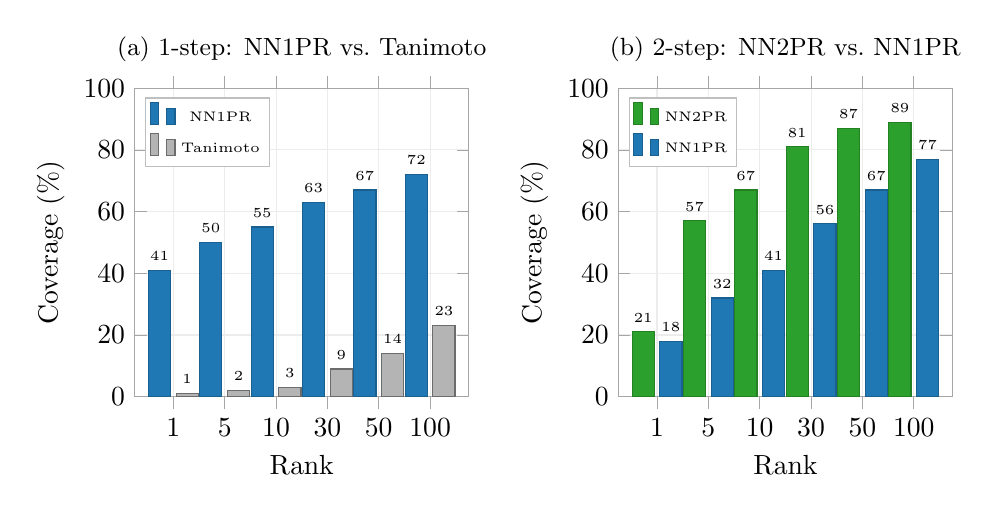
\begin{tikzpicture}
\begin{axis}[
    name=ax1,
    title style={at={(0.5,1.0)}, anchor=south, font=\small},
    title={(a) 1-step: NN1PR vs.\ Tanimoto},
    ybar,
    bar width=8pt,
    width=0.48\textwidth,
    height=5.5cm,
    ylabel={Coverage (\%)},
    xlabel={Rank},
    symbolic x coords={1,5,10,30,50,100},
    xtick=data,
    ymin=0, ymax=100,
    ytick={0,20,40,60,80,100},
    legend style={at={(0.03,0.97)}, anchor=north west, font=\tiny, draw=gray!50, inner sep=1.5pt, row sep=0.5pt},
    nodes near coords,
    every node near coord/.append style={font=\tiny},
    enlarge x limits=0.15,
    grid=major,
    grid style={gray!15},
    axis line style={gray!70},
    tick style={gray!70},
]
\addplot[fill=nn1prcolor, draw=nn1prcolor!80!black] coordinates {(1,41) (5,50) (10,55) (30,63) (50,67) (100,72)};
\addplot[fill=tanimotocolor, draw=tanimotocolor!60!black] coordinates {(1,1) (5,2) (10,3) (30,9) (50,14) (100,23)};
\legend{NN1PR, Tanimoto}
\end{axis}

\begin{axis}[
    at={(ax1.outer east)},
    anchor=outer west,
    xshift=0.2cm,
    title style={at={(0.5,1.0)}, anchor=south, font=\small},
    title={(b) 2-step: NN2PR vs.\ NN1PR},
    ybar,
    bar width=8pt,
    width=0.48\textwidth,
    height=5.5cm,
    ylabel={Coverage (\%)},
    xlabel={Rank},
    symbolic x coords={1,5,10,30,50,100},
    xtick=data,
    ymin=0, ymax=100,
    ytick={0,20,40,60,80,100},
    legend style={at={(0.03,0.97)}, anchor=north west, font=\tiny, draw=gray!50, inner sep=1.5pt, row sep=0.5pt},
    nodes near coords,
    every node near coord/.append style={font=\tiny},
    enlarge x limits=0.15,
    grid=major,
    grid style={gray!15},
    axis line style={gray!70},
    tick style={gray!70},
]
\addplot[fill=nn2prcolor, draw=nn2prcolor!80!black] coordinates {(1,21) (5,57) (10,67) (30,81) (50,87) (100,89)};
\addplot[fill=nn1prcolor, draw=nn1prcolor!80!black] coordinates {(1,18) (5,32) (10,41) (30,56) (50,67) (100,77)};
\legend{NN2PR, NN1PR}
\end{axis}
\end{tikzpicture}
